%%%%%%%%%%%%%%%%%%%%%%%%%%%%%%%%%
%%%%%%%% d(q,tau) vs tau
\begin{frame}
	\begin{tikzpicture}[remember picture,overlay]
	\fill[blue1]
	(current page.north west) rectangle ([xshift=0.52\paperwidth,yshift=0.33\paperheight]current page.west|-{pic cs:end});
	\end{tikzpicture}
	
	\begin{textblock}{0.6}(0.02,0.03)
		\textcolor{white}{
			\Large The image structure function $D(q, \tau)$}
	\end{textblock}

	\begin{textblock}{0.44}(0.02,0.1)
	\includegraphics[width=\textwidth]
	{Sources/X-DFA/img_struc_func_vs_q_multiple_tau_simulations_nPart10Marker.eps}
	\end{textblock}

	\begin{textblock}{0.44}(0.52,0.1)
	\only<1>{
	\includegraphics[width=\textwidth]
	{Sources/X-DFA/img_struc_func_vs_tau_q_range_000simulations10.pdf}}

	\only<2>{
	\includegraphics[width=\textwidth]
	{Sources/X-DFA/img_struc_func_vs_tau_q_range_001simulations10.pdf}}

	\only<3>{
	\includegraphics[width=\textwidth]
	{Sources/X-DFA/img_struc_func_vs_tau_q_range_002simulations10.pdf}}

	\visible<4->{
	\includegraphics[width=\textwidth]
	{Sources/X-DFA/img_struc_func_vs_tau_q_range_007simulations10.pdf}}
	\end{textblock}


	\begin{textblock}{0.5}(0.02,0.63)
	\only<4>{\small
	\begin{align}
	D(q,\tau)
	&= \Big\langle |I(q, t+\tau) - I(q,t)|^2  \Big\rangle_t \nonumber \\
	&= A(q) 
	\left[1-\frac{\big\langle I^*(q,t) I(q,t+\tau) \big\rangle_t}
	{\big\langle |I(q,t)|^2 \big\rangle_t}\right] 
	+ B(q)\nonumber
	\end{align}
	}
	\visible<5->{\small
	\begin{align}
	D(q,\tau)
	&= \Big\langle |I(q, t+\tau) - I(q,t)|^2  \Big\rangle_t \nonumber \\
	&= A(q) 
	\bigg[1-
	\textcolor{red}{\underbrace{
			\frac{\big\langle I^*(q,t) I(q,t+\tau) \big\rangle_t}
			{\big\langle |I(q,t)|^2 \big\rangle_t}
	}}
	\bigg] 
	+ B(q)\nonumber
	\end{align}
	}
	\end{textblock}

	\begin{textblock}{0.3}(0.2,0.92)
	\visible<5->{
		\textcolor{red}{Image correlation function}
	}
	\end{textblock}

%	\begin{textblock}{0.5}(0.52,0.68)
%	\visible<6>{
%	\centering
%	\colorbox{lightblue}{
%	Linear space invariant imaging}
%	\small
%	\begin{align}
%	f(q,\tau) = \frac
%	{\langle \rho^*(q,t) \rho(q,t+\tau) \rangle_t}
%	{\langle |\rho(\mathbf{q},t)|^2 \rangle_t}
%	\nonumber
%	\end{align}
%
%	\normalsize
%	Intermediate scattering function
%	}
%	\end{textblock}
\end{frame}




\begin{frame}[noframenumbering]
\begin{textblock}{0.38}(0.02,0.02)
	\only<1>{
	\includegraphics[width=\textwidth]
	{Sources/X-DFA/img_struc_func_vs_q_Ntau999_nPart10.pdf}}

	\visible<2->{
	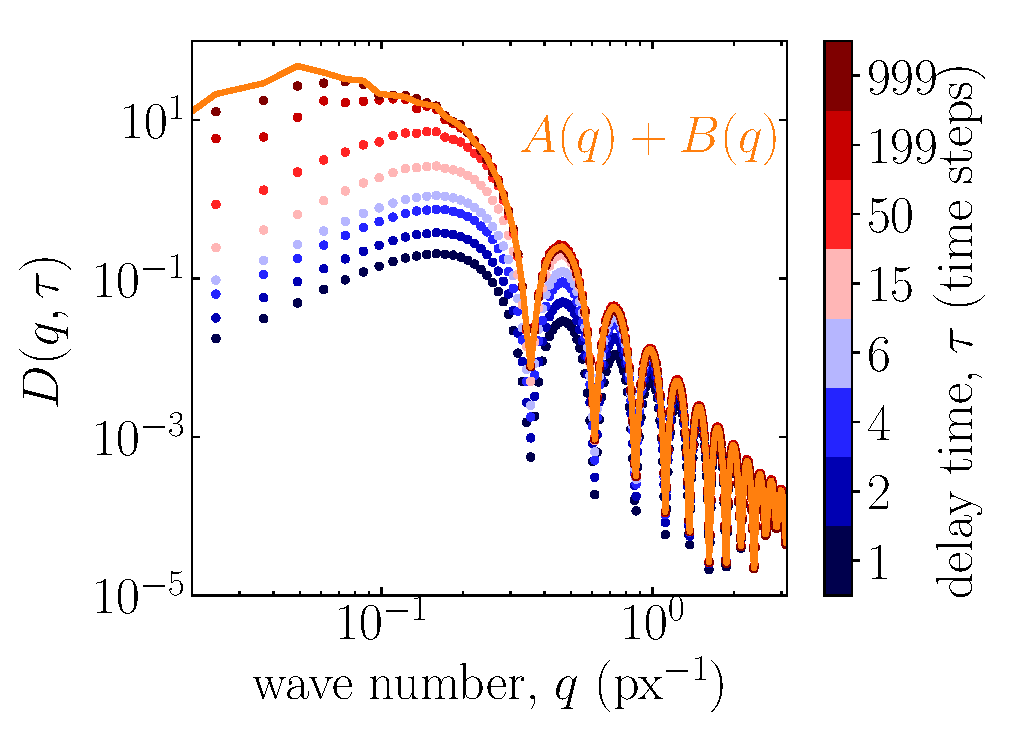
\includegraphics[width=\textwidth]
	{Sources/X-DFA/img_struc_func_vs_q_multiple_tau_simulations_nPart10with_A.eps}}
\end{textblock}

\begin{textblock}{0.38}(0.55,0.02)
	\visible<1->{
		\includegraphics[width=\textwidth]
		{Sources/X-DFA/img_struc_func_vs_tau_q_range_007simulations10.pdf}}
\end{textblock}



\begin{textblock}{0.5}(0.02,0.5)
	\only<1>{
	\begin{align}
	D(q,\tau)
	&= \Big\langle |I(q, t+\tau) - I(q,t)|^2  \Big\rangle_t \nonumber \\
	&= A(q) 
	\bigg[1-
	\textcolor{red}{\underbrace{
			\frac{\big\langle I^*(q,t) I(q,t+\tau) \big\rangle_t}
			{\big\langle |I(q,t)|^2 \big\rangle_t}
	}}
	\bigg] 
	+ B(q)\nonumber
	\end{align}
	}
\end{textblock}

\begin{textblock}{0.3}(0.2,0.8)
	\only<1>{
		\textcolor{red}{Image correlation function}
	}
\end{textblock}

\begin{textblock}{0.5}(0.02,0.5)
	\visible<2->{
		\begin{align}
		D(q,\tau)
		&= \Big\langle |I(q, t+\tau) - I(q,t)|^2  \Big\rangle_t \nonumber \\
		&= \textcolor{orange}{A(q)}
		\bigg[1-
		\textcolor{red}{
				\frac{\big\langle I^*(q,t) I(q,t+\tau) \big\rangle_t}
				{\big\langle |I(q,t)|^2 \big\rangle_t}
		}
		\bigg] 
		+ \textcolor{darkgreen}{B(q)}\nonumber
		\end{align}
		
	\begin{itemize}
		\item $D(q, \tau \rightarrow 0) = \textcolor{darkgreen}{B(q)} = 0$
		\item $D(q, \tau \rightarrow \infty) = \textcolor{orange}{A(q) + B(q)}$
	\end{itemize}
	}
\end{textblock}

\begin{textblock}{0.5}(0.52,0.55)
	\only<1,2>{
	\centering
	\colorbox{lightblue}{
		Linear space invariant imaging}
	\begin{align}
	f(q,\tau) = \frac
	{\langle \rho^*(q,t) \rho(q,t+\tau) \rangle_t}
	{\langle |\rho(q,t)|^2 \rangle_t}
	\nonumber
	\end{align}
	
	Intermediate scattering function}
\end{textblock}


\begin{textblock}{0.38}(0.55,0.5)
	\visible<3->{
		\includegraphics[width=\textwidth]
		{Sources/X-DFA/ISF_vs_tau.eps}}
\end{textblock}
\end{frame}